\documentclass{beamer}
\usepackage[utf8]{inputenc}

\usetheme{Madrid}
\usecolortheme{default}
\usepackage{amsmath,amssymb,amsfonts,amsthm}
\usepackage{txfonts}
\usepackage{tkz-euclide}
\usepackage{listings}
\usepackage{adjustbox}
\usepackage{array}
\usepackage{tabularx}
\usepackage{gvv}
\usepackage{lmodern}
\usepackage{circuitikz}
\usepackage{lmodern}
\usepackage{multicol}
\usepackage{tikz}
\usepackage{graphicx}

\setbeamertemplate{page number in head/foot}[totalframumber]

\usepackage{tcolorbox}
\tcbuselibrary{minted,breakable,xparse,skins}



\definecolor{bg}{gray}{0.95}
\DeclareTCBListing{mintedbox}{O{}m!O{}}{%
  breakable=true,
  listing engine=minted,
  listing only,
  minted language=#2,
  minted style=default,
  minted options={%
    linenos,
    gobble=0,
    breaklines=true,
    breakafter=,,
    fontsize=\small,
    numbersep=8pt,
    #1},
  boxsep=0pt,
  left skip=0pt,
  right skip=0pt,
  left=25pt,
  right=0pt,
  top=3pt,
  bottom=3pt,
  arc=5pt,
  leftrule=0pt,
  rightrule=0pt,
  bottomrule=2pt,
  toprule=2pt,
  colback=bg,
  colframe=orange!70,
  enhanced,
  overlay={%
    \begin{tcbclipinterior}
    \fill[orange!20!white] (frame.south west) rectangle ([xshift=20pt]frame.north west);
    \end{tcbclipinterior}},
  #3,
}
\lstset{
    language=C,
    basicstyle=\ttfamily\small,
    keywordstyle=\color{blue},
    stringstyle=\color{orange},
    commentstyle=\color{green!60!black},
    numbers=left,
    numberstyle=\tiny\color{gray},
    breaklines=true,
    showstringspaces=false,
}
%------------------------------------------------------------
%This block of code defines the information to appear in the
%Title page
\title %optional
{8.4.5}
\date{October 5,2025}
%\subtitle{A short story}

\author % (optional)
{EE25BTECH11002 - Achat Parth Kalpesh}



\begin{document}


\frame{\titlepage}

\begin{frame}{Question}
An ellipse is drawn by taking a diameter of the circle $\brak{x-1}^2+y^2=1$ as its semi minor axis and a diameter of the circle $x^2+\brak{y-2}^2=4$ as semi-major axis. If the centre of the ellipse is at the origin and its axes are the coordinate axes, then the equation of the ellipse is 
\begin{multicols}{2}
\begin{enumerate}
    \item $4x^2+y^2=4$ 
    \item $x^2+4y^2=8$
    \item $4x^2+y^2=8$
    \item $x^2+4y^2=1$
\end{enumerate}
\end{multicols}
\end{frame}

\begin{frame}{Solution}
The standard equation of a circle is given as
\begin{align}
    \brak{\vec{x}-\vec{c}}^\top\brak{\vec{x}-\vec{c}} = r^2
\end{align}

Given two circles are
\begin{align}
    \brak{\vec{x}-\vec{c_1}}^\top\brak{\vec{x}-\vec{c_1}} = 1\\
    \brak{\vec{x}-\vec{c_2}}^\top\brak{\vec{x}-\vec{c_2}} = 4
\end{align}

The centers and radii are
\begin{align}
    \vec{c_1} = \myvec{1\\0}, \quad r_1 = 1\\
    \vec{c_2} = \myvec{0\\2}, \quad r_2 = 2
\end{align}
\end{frame}



\begin{frame}{Solution}
Verifing that the origin lies on both circles:
\begin{align}
    \brak{\vec{0}-\vec{c_1}}^\top\brak{\vec{0}-\vec{c_1}} = 1 = r_1^2\\
    \brak{\vec{0}-\vec{c_2}}^\top\brak{\vec{0}-\vec{c_2}} = 4 = r_2^2
\end{align}

Thus, the diameters of both circles passing through the origin are along the directions
\begin{align}
    \vec{c_1} = \myvec{1\\0} \text{ \brak{\text{along X-axis}}}\\
    \vec{c_2} = \myvec{0\\2} \text{ \brak{\text{along Y-axis}}}
\end{align}
\end{frame}

\begin{frame}{Solution}
Each circle's diameter length is $2r$. Therefore, the ellipse's 
semi-axes are equal to the respective radii:
\begin{align}
    b = r_1 = 1 \quad \text{\brak{\text{semi-minor axis}}}\\
    a = r_2 = 2 \quad \text{\brak{\text{semi-major axis}}}
\end{align}
The standard equation of an ellipse centered at the origin with coordinate axes as its axes is
\begin{align}
    \vec{x}^\top A \vec{x} = 1
\end{align}
where
\begin{align}
    A = \myvec{\frac{1}{b^2} & 0 \\ 0 & \frac{1}{a^2}}
\end{align}
\end{frame}

\begin{frame}{Solution}
Substituting $a = 2,\, b = 1$,
\begin{align}
    A = \myvec{1 & 0 \\ 0 & \frac{1}{4}}
\end{align}
Hence,
\begin{align}
    \vec{x}^\top\myvec{1 & 0 \\ 0 & \frac{1}{4}}\vec{x} = 1
\end{align}

Multiplying throughout by $4$ gives
\begin{align}
    \vec{x}^\top\myvec{4 & 0 \\ 0 & 1}\vec{x} = 4
\end{align}

or equivalently,
\begin{align}
    4x^2 + y^2 = 4
\end{align}
\end{frame}
\begin{frame}{Python Plot}
    \begin{figure}
        \centering
        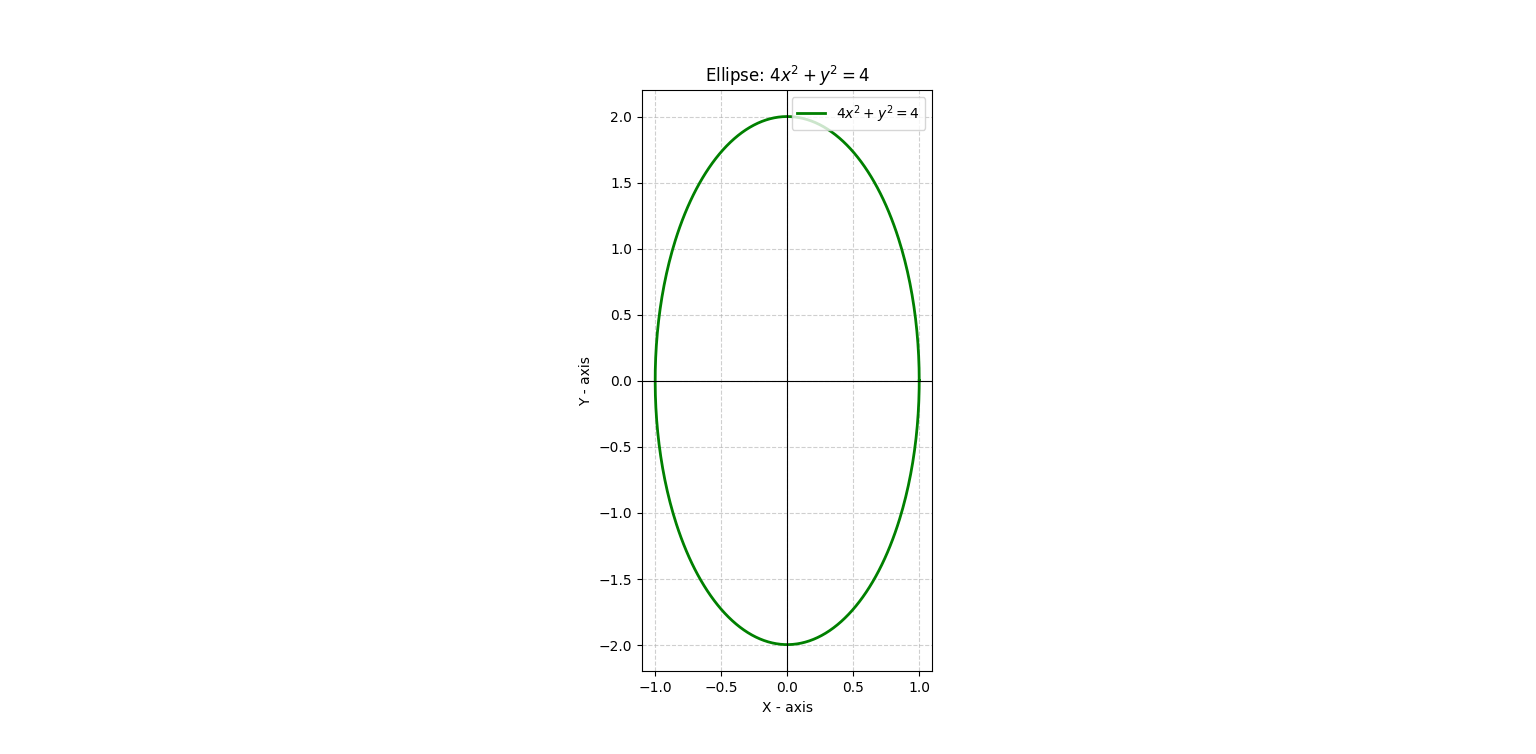
\includegraphics[width=\columnwidth]{../figs/figure_py.png}
        \caption{Ellipse}
        \label{fig:fig}
    \end{figure}
\end{frame}
\end{document}
